
\documentclass[12pt]{article}
\usepackage{graphicx} % for including images
\usepackage{hyperref} % for creating hyperlinks
\usepackage{amsmath} % for mathematical expressions
\usepackage{lipsum} % for generating dummy text
\usepackage{listings} % for code blocks
\usepackage{float} % place images where they appear in the LaTeX

\lstset{
  language=bash,
  basicstyle=\ttfamily,
  breaklines=true
}

\begin{document}
% Title page information
\title{Does the Raspberry Pi 4B Have a GPGPU?}
\author{Jaidon Lybbert, University of Washington}
\date{January 24, 2024}

% Generate the title page
\maketitle

% Abstract section
\begin{abstract}
The Raspberry Pi 4B uses the Broadcomm BCM2711 SoC, which features a quad-core ARM Cortex-A72 CPU, and a Broadcomm VideoCore VI GPU. The VideoCore VI GPU is purpose-built for graphics applications, and there is very limited support for directly programming the device from the manufacturer. The focus of this article is to investigate the capabilities of the VideoCore GPU for General Purpose GPU (GPGPU) tasks, that is, compute tasks not involving graphics. Several open-source methods of programming are evaluated, and performance of the GPU is benchmarked against the CPU for the General Matrix Multiply (GEMM) algorithm extensively used in machine learning and machine vision applications.
\end{abstract}

% Introduction section
\section{Introduction}
This document is organized as follows. In Section \ref{sec:background} I describe my experience with embedded systems and software, motivations and intent. I describe the setup of my environment in Section \ref{sec:methods} and perform some benchmarking tests. I show the benchmark results in Section \ref{sec:results}, and discuss the results along with the failures and hurdles I faced in Section \ref{sec:discussion}. I conclude in \ref{sec:conclusion} by discussing the improvements I would like to make in the future.

% Methods section
\section{Background}\label{sec:background}

\subsection{GPUs and GPGPUs}
As clock rates stopped increasing, and Moore's law began to taper off, parallel processers emerged to increase compute throughput by allowing some algorithms to be broken down into pieces that could be solved simeoultaneously. Fueled by the \verb|$300B| gaming industry, parallel processors have rapidly taken over for video-encoding and decoding in computers and mobile phones. Nearly anything displaying to a screen now has a graphics processor. The emergence of AI training and inference has created new demand for General Purpose GPUs (GPGPUs) which are not restricted to graphics processing, but can be easily programmed for other compute tasks. NVIDIAs CUDA platform is built for this market, making programming their family of GPUs easy by providing a language, compiler, and debugging tools that integrate with existing languages and tools like C++, and Visual Studio.

Machine vision algorithms like Simultaneous Localization And Mapping (SLAM), and other applications, demand portable GPGPUs which can be programmed with arbitrary code and be integrated into a small portable device to perform parallel processing. The NVIDIA Jetson family of devices is tailored to this market, offering scaled down chips, and development boards for embedded programmers as low as \verb|$130|.

In this article, we will look at the GPU on the Raspberry Pi. A device which, as we'll see, was clearly not intended to be used as a GPGPU. However, recent developments in software drivers and graphics APIs just might enable this device to massively speed up some compute workloads. 

\subsection{VideoCore IV and VI}
The Broadcomm chips in the Raspberry Pis have VideoCore GPUs. The Raspberry Pi 1, 2, and 3 have the VideoCore IV GPU, and the Raspberry Pi 4 has the VideoCore VI GPU. The VideoCore IV is also found in devices such as the Roku, Amazon Fire TV Stick, and phones from Samsung, Nokia, and Apple's iPod. 

We will focus on the BCM2711 SoC featured in the Raspberry Pi 4B, which has a VideoCore VI GPU. 

\subsection{Setting the Baseline}
To evaluate the performance of the VideoCore VI GPU, there are two useful comparisons: 

\begin{itemize}
\item How does it perform compared to the CPU on-chip?
\item How does it perform compared to an NVIDIA Jetson?
\end{itemize}

The first question is arguably more relevant to someone who already has a Raspberry Pi. After all, why go through the trouble if the CPU is faster anyway?

The second question is really asking, is it ever a good idea to buy a Raspberry Pi for GPGPU-related tasks? 

\subsection{Motivation}
Two big questions motivate my research: ``what is the performance of the VideoCore VI GPU?'' and ``how do I program it?''

This small list of large questions breaks down into a large list of smaller questions.

\begin{itemize}
  \item What is the compute throughput of the VideoCore VI GPU?
  \item How do instructions map to hardware?
  \item How many parallel threads does the GPU support?
  \item What other APIs exist for GPU programming?
  \item Previous work done and results
  \item What is the memory model for the GPU + CPU?
  \item CPU and GPU caching?
  \item Supported language bindings?
  \item Memory latency?
\end{itemize}

\subsection{Prior Works}

Broadcomm has not released much documentation for the VideoCore VI GPU. Much of the information about the GPU is derived from the previous VideoCore IV reference manual \cite{videocoreiv}, which Broadcomm did release, and open-source drivers written with the help of Broadcomm engineers in the Linux kernel repository \cite{torvalds_linux_2024}, and the MESA graphics library \cite{external-mesa}. 

Various projects over the years have attempted to make programming the GPUs easier on the Raspberry Pi. 

The GitHub user ``hermanhermitage'' investigated the VideoCore IV GPU, and created a wiki their findings \cite{videocoreiv_herman}. They used US patent applications filed by Broadcomm along with experimentation to characterize the architecture, memory layout, instruction set, and registers for the device. The project includes a guide on intercepting GPU execution by replacing the \verb|bootcode.bin| in the boot partition of the SD card. Broadcomm eventually published a full specification for the VideoCore IV, superceding this effort with official documentation.

QPULib is a C++ library by Matthew Naylor for compiling and offloading programs for the VideoCore IV GPU (Raspberry Pi versions 1, 2, 3) during runtime \cite{QPULib}. Efforts by Wim Rijnders extended this idea to the VideoCore VI in the Raspberry Pi 4, with the C++ library V3DLib \cite{rijnders2021v3dlib}. V3DLib depends on the Mesa graphics library for disassembly of VideoCore instructions. It's worth noting that neither of these projects have had active development in the last 3 years, and support for new OS versions is unknown. 

A totally separate project, \verb|py-videocore6| \cite{pyvideocore6}, is a Python library enabling the programming of the VideoCore VI through the Direct Rendering Manager (DRM) graphics driver in the Linux kernel.

The Raspberry Pi Foundation recently announced that the Raspberry Pi 4 is now Vulkan 1.2 compliant through the Mesa graphics driver. This was a joint effort by Raspberry Pi, Mesa, and Broadcomm developers. Vulkan is a graphics library, which in contrast to older graphics libraries like OpenGL ES, supports an efficient compute-only pipeline, without any involvement of the framebuffer. Vulkan has been getting used more recently in machine learning applications for its cross-platform support. However, the Vulkan 1.2 specification does allow many features to be optional, so it isn't clear to what extent compute can be done through Vulkan until it is installed and queried for the supported features.

\section{Methods}\label{sec:methods}
In order to make any meaningful observations about the capability of the Broadcomm VideoCore VI GPU on the Raspberry Pi 4B, I will compare the programming experience and capabilities of the device to the widely used NVIDIA CUDA platform. Obviously, with the NVIDIA chips being orders of magnitude more expensive, they have many more cores and features, but on a core-to-core basis they are similar SIMD processors with similar function. For comparisons sake, I will show how the \verb|$35| 2GB Raspberry Pi 4B \textbf{theoretically} stacks against the \verb|$600| 11GB NVIDIA GTX 2080 TI graphics card at scale in terms of power consumption, compute throughput, and memory bandwidth.

\subsection{CUDA Overview}
Through my graduate research, I studied parallel computing using the NVIDIA Cuda toolkit on NVIDIA GPU architectures. The Turing Streaming Multiprocessor (SM) architecture featured in the RTX 20xx family of GPUs features Tensor Core hardware units for performing tensor calculations using reduced precision data types including IEEE-754 FP16, and unsigned 8-bit integers. Each SM can perform 1024 FP16 fused multiply accumulate (FMA) operations per clock cycle, or 2048 INT8 FMA operations. With 68 SMs on a consumer-grade chip (RTX 2080 Ti), that means 69k FMA operations per clock cycle, giving it an FP16 compute throughput of 

\subsection{CPU GMEM Benchmarks}

As a benchmark, I chose to use a naive matrix multiply algorithm, as it has the potential to be memory-bound or compute-bound, and is easy to implement and analyze. The algorithmic complexity is O(n\textasciicircum3). For the basic CPU version, I use Bing AI to generate the algorithm in Rust which iterates over many matrix sizes, and records their execution times to a \verb|.csv| file. I then use Bing AI to generate a Python function to plot the results from the \verb|.csv| file.

% Results section
\section{Results}\label{sec:results}

\subsection{Cortex-A72 Characterization}

The ARM Cortex-A72 CPU is thoroughly documented by ARM, with a public reference manual \cite{ARM2021}. Details specific to the Raspberry Pi 4B are published in the Raspberry Pi documentation \cite{raspberrypi2024}. The relevant high-level details are summarized here.

Quad-core Cortex-A72 64-bit @ 1.5 GHz

\subsubsection{Memory}

\begin{itemize}
\item 4GB LPDDR4-2400 SDRAM
\item 32kB data + 48kB instruction L1 cache per core
\item 1MB L2 cache
\end{itemize}

\subsubsection{CPU Architecture}

The Cortex-A72 CPU in the Raspberry Pi 4B has 4 cores, each with 32kB data cache and 48kB instruction cache. The cores share a 1MB L2 cache.

The CPU supports SIMD operations.

ACE, CHI interface.

Translation Lookaside Buffer (TLB)

\begin{figure}[h]
\centering
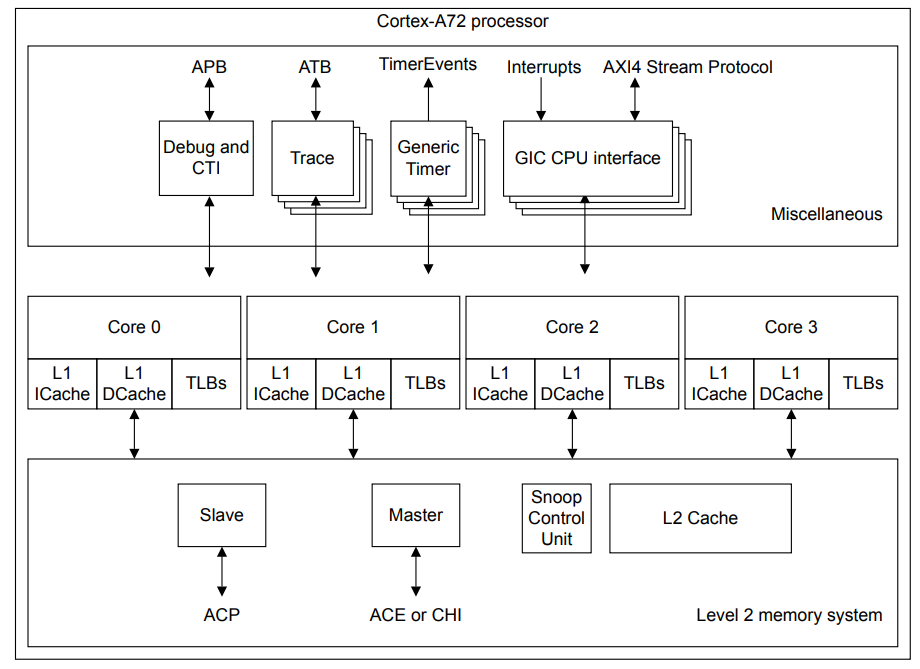
\includegraphics[width=1.0\textwidth]{A72_Core_Diagram.png} % replace with your own image file
\caption{Block diagram of the quad-core ARM Cortex-A72 CPU.}
\label{fig:A72_arch}
\end{figure}

\subsubsection{Throughput}

\subsection{VideoCore VI Characterization}

VideoCore VI 32-bit @ 500 MHz.
MMU.

\subsection{Programming}

\subsubsection{V3DLib}

V3DLib is a language and compiler for the VideoCore VI GPU created by Wim Rjinder's in C++. The project has a large number of dependencies, and ultimately uses the Mesa graphics library to translate code to run on the device. Because of the large number of dependencies and stale development (hasn't been updated in 3 years), it may be prohibitively difficult to use this method of programming. 

I cloned the repository and ran the build script.
	
\begin{lstlisting}
> sudo apt-get install git                                     
> sudo apt install libexpat1-dev                                
> git clone --depth 1 https://github.com/wimrijnders/V3DLib.git  
> cd V3DLib
> make QPU=1 DEBUG=1 all                                
\end{lstlisting}

The build failed due to missing headers, which I found were included in the raspberry pi development headers

\subsubsection{pyvideocore6}

\subsubsection{Vulkan 1.2}

% Discussion section
\section{Discussion}\label{sec:discussion}

% Conclusion section
\section{Conclusion}\label{sec:conclusion}
\paragraph{Note}
\textit{All my code and project files for this and future reports, can be found on my GitHub repository \cite{lybbert2024classwork}.}

% Bibliography from refs.bib
\bibliographystyle{plain}
\bibliography{refs}

\end{document}
